%%%%%%%%%%%%%%%%%%%%%%%%%%%%%%%%%%%%%%%%%
% Large Colored Title Article
% LaTeX Template
% Version 1.1 (25/11/12)
%
% This template has been downloaded from:
% http://www.LaTeXTemplates.com
%
% Original author:
% Frits Wenneker (http://www.howtotex.com)
%
% License:
% CC BY-NC-SA 3.0 (http://creativecommons.org/licenses/by-nc-sa/3.0/)
%
%%%%%%%%%%%%%%%%%%%%%%%%%%%%%%%%%%%%%%%%%

%----------------------------------------------------------------------------------------
%	PACKAGES AND OTHER DOCUMENT CONFIGURATIONS
%----------------------------------------------------------------------------------------

\documentclass[DIV=calc, paper=a4, fontsize=10pt, twocolumn]{scrartcl}\usepackage[]{graphicx}\usepackage[]{color}
%% maxwidth is the original width if it is less than linewidth
%% otherwise use linewidth (to make sure the graphics do not exceed the margin)
\makeatletter
\def\maxwidth{ %
  \ifdim\Gin@nat@width>\linewidth
    \linewidth
  \else
    \Gin@nat@width
  \fi
}
\makeatother

\definecolor{fgcolor}{rgb}{0.345, 0.345, 0.345}
\newcommand{\hlnum}[1]{\textcolor[rgb]{0.686,0.059,0.569}{#1}}%
\newcommand{\hlstr}[1]{\textcolor[rgb]{0.192,0.494,0.8}{#1}}%
\newcommand{\hlcom}[1]{\textcolor[rgb]{0.678,0.584,0.686}{\textit{#1}}}%
\newcommand{\hlopt}[1]{\textcolor[rgb]{0,0,0}{#1}}%
\newcommand{\hlstd}[1]{\textcolor[rgb]{0.345,0.345,0.345}{#1}}%
\newcommand{\hlkwa}[1]{\textcolor[rgb]{0.161,0.373,0.58}{\textbf{#1}}}%
\newcommand{\hlkwb}[1]{\textcolor[rgb]{0.69,0.353,0.396}{#1}}%
\newcommand{\hlkwc}[1]{\textcolor[rgb]{0.333,0.667,0.333}{#1}}%
\newcommand{\hlkwd}[1]{\textcolor[rgb]{0.737,0.353,0.396}{\textbf{#1}}}%

\usepackage{framed}
\makeatletter
\newenvironment{kframe}{%
 \def\at@end@of@kframe{}%
 \ifinner\ifhmode%
  \def\at@end@of@kframe{\end{minipage}}%
  \begin{minipage}{\columnwidth}%
 \fi\fi%
 \def\FrameCommand##1{\hskip\@totalleftmargin \hskip-\fboxsep
 \colorbox{shadecolor}{##1}\hskip-\fboxsep
     % There is no \\@totalrightmargin, so:
     \hskip-\linewidth \hskip-\@totalleftmargin \hskip\columnwidth}%
 \MakeFramed {\advance\hsize-\width
   \@totalleftmargin\z@ \linewidth\hsize
   \@setminipage}}%
 {\par\unskip\endMakeFramed%
 \at@end@of@kframe}
\makeatother

\definecolor{shadecolor}{rgb}{.97, .97, .97}
\definecolor{messagecolor}{rgb}{0, 0, 0}
\definecolor{warningcolor}{rgb}{1, 0, 1}
\definecolor{errorcolor}{rgb}{1, 0, 0}
\newenvironment{knitrout}{}{} % an empty environment to be redefined in TeX

\usepackage{alltt}	 % A4 paper and 11pt font size

\usepackage{lipsum} % Used for inserting dummy 'Lorem ipsum' text into the template
\usepackage{url}
\usepackage{natbib}
\usepackage[english]{babel} % English language/hyphenation
\usepackage[protrusion=true,expansion=true]{microtype} % Better typography
\usepackage{amsmath,amsfonts,amsthm} % Math packages
\usepackage[svgnames]{xcolor} % Enabling colors by their 'svgnames'
\usepackage[hang, small,labelfont=bf,up,textfont=it,up]{caption} % Custom captions under/above floats in tables or figures
\usepackage{booktabs} % Horizontal rules in tables
\usepackage{fix-cm}	 % Custom font sizes - used for the initial letter in the document
\usepackage{natbib}
\usepackage{sectsty} % Enables custom section titles
\allsectionsfont{\usefont{OT1}{phv}{b}{n} \fontsize{12}{12}} % Change the font of all section commands
\usepackage{hyperref}
\usepackage{float}
\usepackage{fancyhdr} % Needed to define custom headers/footers
\pagestyle{fancy} % Enables the custom headers/footers
\usepackage{lastpage} % Used to determine the number of pages in the document (for "Page X of Total")

% Headers - all currently empty
\lhead{}
\chead{\emph{Vizualizing the African Slave Trade, 1514 - 1866}}
\rhead{}

% Footers
\lfoot{}
\cfoot{}
\rfoot{\footnotesize Page \thepage\ of \pageref{LastPage}} % "Page 1 of 2"

\renewcommand{\headrulewidth}{0.0pt} % No header rule
\renewcommand{\footrulewidth}{0.4pt} % Thin footer rule

\usepackage{lettrine} % Package to accentuate the first letter of the text
\newcommand{\initial}[1]{ % Defines the command and style for the first letter
\lettrine[lines=3,lhang=0.3,nindent=0em]{
\color{black}
{\textsf{#1}}}{}}
\usepackage{color}
\definecolor{purple}{rgb}{.4,0,.8}
\newcommand{\hh}[1]{{\color{magenta} #1}}
\newcommand{\st}[1]{{\color{purple} #1}}

%----------------------------------------------------------------------------------------
%	TITLE SECTION
%----------------------------------------------------------------------------------------

\usepackage{titling} % Allows custom title configuration

\newcommand{\HorRule}{\color{black} \rule{\linewidth}{1pt}} % Defines the gold horizontal rule around the title

\pretitle{\vspace{-50pt} \begin{flushleft} \HorRule \fontsize{15}{15} \usefont{OT1}{phv}{b}{n} \color{black} \selectfont} % Horizontal rule before the title

\title{Using the \texttt{geomnet} Package: Visualizing African Slave Trade, 1514 - 1866} % Your article title
 % This should probably reference geomnet. Don't want it to be too long though
\posttitle{\par\end{flushleft}\vskip 0em} % Whitespace under the title

\preauthor{\begin{flushleft}\large \vspace{-.5cm} \usefont{OT1}{phv}{b}{sl} \color{black}} % Author font configuration

\author{Sam Tyner, } % Your name

\postauthor{\footnotesize \usefont{OT1}{phv}{m}{sl} \color{Black} % Configuration for the institution name
Iowa State University % Your institution

\par\end{flushleft} \vspace{-.5cm} \HorRule \vspace{-1cm}} % Horizontal rule after the title
\date{} % Add a date here if you would like one to appear underneath the title block

%----------------------------------------------------------------------------------------
\IfFileExists{upquote.sty}{\usepackage{upquote}}{}
\begin{document}

\maketitle % Print the title

\thispagestyle{fancy} % Enabling the custom headers/footers for the first page 

%----------------------------------------------------------------------------------------
%	ABSTRACT
%----------------------------------------------------------------------------------------

% The first character should be within \initial{}
\vspace{-1cm}
%\initial{U}\textbf{sing a new way to visualize network data in \texttt{R} with \texttt{gglot2}, I examine the evolution of the African slave trade from the $16^{th}$ through the $19^{th}$ centuries. \st{XXX I feel like I need more here. Will add more when paper is more fleshed out.}}

%\initial{T}\textbf{he Trans-Atlantic Slave Trade Database, hosted by Emory University, contains information on nearly 35,000 voyages of slave ships from 1514 - 1866 between Europe, Africa, and the Americas. The entire database contains 279 variables with information on the 34,948 voyages. While the website dedicated to this data contains a dashboard to subset and visualize the data, I wanted to view the data in a new way. I use the \texttt{geomnet} package because I wanted to show that the user can visually explore the data in a way that leaves them with a deeper understanding of the structure of the slave trade. I start by visualizing all of the data I pulled from the database on one map, then I look at different subsets of it, and I end with a much deeper understanding of the slave trade and its impact on the world.}
%----------------------------------------------------------------------------------------
%	ARTICLE CONTENTS
%----------------------------------------------------------------------------------------
\section*{Introduction}

\par The Trans-Atlantic Slave Trade Database, hosted by Emory University, contains information on nearly 35,000 voyages of slave ships from 1514 - 1866 between Europe, Africa, and the Americas.%\citep{voyages}
The data are extensive, and come chiefly from primary sources, such as ship manifests or family and business records. Although the current host of these data is Emory University, collecting this vital historic data has taken decades. In the last 15 years alone, over 50 individual researchers have contributed data from their own research to help complete this database. 

\par The entire database contains 279 variables with information on the 34,948 voyages. Some of the variables included in the database are the ships' owners, the country of origin of the ship, the number of men, women, and children that were taken from Africa, and the outcome of the voyage. The database also includes information on ships that were wrecked, captured, or never heard from again. For my visualizations, I only include trips with outcomes that were completed as planned, where slaves disembarked in the Americas or disembarked in Africa or Europe.  Additionally, due to the inconsistent nature of the historical data sources, there are many missing values, and 22 of the 279 variables are actually imputed.\footnote{See \url{http://www.slavevoyages.org/voyage/understanding-db/methodology-9} for more information on how the imputed variables are derived.} In order to fully appreciate the magnitude of this data, I use the imputed varibles because they contain the most information about the trans-Atlantic slave trade. By using the most robust variables, I can present the most complete visual analysis of the forced migration of Africans to the Americas.  

\par The website dedicated to exploring this data, \url{https://www.slavevoyages.org}, contains a dashboard to view and subset the data. It also hosts a graph builder for simple plots, such as scatterplots, time series, or bar graphs, as well as an interactive map and an animation of all slave ships leaving Africa and arriving in the Americas. While using these tools, I felt that the interactive map lacked detail and flexibility. It is possible for the user to zoom in to see more detail, but by zooming in, you lose the entire journey and can only focus on one port or one subregion at a time. There is not a way to view all the voyages individually on the map. The animation, which shows slave ships as dots flying across the Atlantic Ocean and arriving in the Americas, is beautiful, but it lacks permanence. Seeing the ships travel across the ocean is very informative, but not very impactful. A similar animiation appeared in Slate Magazine in June 2015.% \citep{slate}.
Neither of these visualizations contain other information about the ships, such as country of the ship or the number of slaves that perished on the journey. Finally, other animations by two researchers at Georgetown University show the cumulative frequencies of port of departure, port of slave purchase, and port of slave sale.% \citep{heatmaps}. 
All of these animations are beautiful, but I think they fail to leave the viewer with a real understanding of the sheer magnitude of this centuries-long practice of taking people from their homes and selling them into slavery in foreign countries.

\par I chose to visualize this data using \texttt{geomnet} because I wanted to show that the user can visually explore it in a way that leaves them with a deeper understanding of the structure of the slave trade. The visuals I created are static and dense: the viewer can examine them for much longer than the animations by Slate Magazine and the others, allowing the user to really sit with the visual and comprehend the severity of the slave trade. I created several visualizations of the Trans-Atlantic Slave Database in order to answer many more questions of interest than the other visualizations answer. A few questions I explore are: Which countries are engaging in the most slave trade? Where are the most slaves being bought and sold? How does the structure of the slave trade change over time? My visualizations give the viewer the ability to begin to answer these questions and more in an easy-to-understand graphic.  
%------------------------------------------------

\section*{The \texttt{geomnet} package}

\par To view the Trans-Atlantic Slave Trade Database in a new way, I use the \texttt{geomnet} package, which can be installed from \url{https://github.com/sctyner/geomnet}.  This package is built on the development version of \texttt{ggplot2}, which can be installed from \url{https://github.com/hadley/ggplot2}.  When the current development version of \texttt{ggplot2} is submitted to \texttt{CRAN}, \texttt{geomnet} will follow closely behind. 

\par The key function in \texttt{geomnet} is a new \texttt{geom} for \texttt{ggplot2}, \texttt{geom\_net()}.  The major advantage of using this new \texttt{geom} over other network packages like \texttt{network} or \texttt{igraph} is the data format required.%\citep{network, igraph}. 
To visualize networks using the current capabilities in those packages, the user needs to be intimately familiar with the structure of network data in these packages and how to manipulate it. The data required for \texttt{geomnet}, however, is just a data frame, like all \texttt{ggplot2} functions require. This is a major advantage for the users who find themselves with network data but have little to no experience with it. 

\par Generally speaking, there are two sets of information in network data: node information and edge information. Node data frames contain the node ids and information on the nodes, such as gender and age of all people in a friendship network, or all employees' departments in a company email network. Edge data frames contain the `from' node id and `to' node id for each each edge, as well as information on the edges, such as length of friendship between two people or time, date, and subject line of an email sent from one person to another. To use \texttt{geom\_net()}, the node and the edge information must be combined into one data frame. The structure of the data frame needed to visualize the network of interest depends on which of these two sets of information the user is primarily interested in visualizing. If the user is focused on node information, they need to perform a full join of the edge and node data by the `from' column of the edge data set and the `id' column of the node data set. If the user is focused on edge information, like I am when visualizing the slave trade data, they need to create two nearly identical rows of data for each edge: the second row is the same as the other with the `from' and `to' nodes reversed. Then, the user should perform the full join of the edge and node data frames. This ensures that all edges and all nodes have their information included in the visualization.   

\par Visualizing networks with \texttt{geom\_net()} will feel very natural to users already familiar with \texttt{ggplot2}. There are several arguments to pass to this function that allow the user to make advanced, customized appearance changes. Some of these arguments are: \texttt{directed}, a value to indicate whether the network is directed or not; \texttt{layout}, a layout algorithm to use if at all; \texttt{arrow}, to change the appearance of directed edges; and \texttt{label}, a character variable of names with which to label nodes. Additionally, there are many more options listed in the package documentation that can be included, like edge and vertex coloring and (x,y) coordinate placement of the nodes that I use in this paper. 

%-----------------------------------------------------------------------------  
% Section : Visualizing the Data




\section*{Visualizing the data}  

I start by visualizing all of the data I pulled from the database on one map. This first visualization, shown in \autoref{fig:whole_dataset_plot}, contains all of the voyages from 1525 - 1864 between Africa and the Americas. This visualization represents voyages that were unwittingly made by 5,095,270 Africans in the 339 years of the trans-Atlantic slave trade. In this first visualization and others, I use the \texttt{colour} and \texttt{group} aesthetic options to color both the nodes and the edges in the network by country of origin of the ships making the voyages. I also use the \texttt{directed = TRUE} option to show that the slaves aboard the ship were brought \emph{from} Africa \emph{to} the Americas. Finally, I use the \texttt{layout = NULL} option and \texttt{x} and \texttt{y} aesthetic options to place the ports in their geographically correct locations. 

\par We can see in \autoref{fig:whole_dataset_plot} that most slaves were brought to islands in the Caribbean, with the most traffic by British, French, and Spanish ships. The two smallest countries involved, Portugal and the Netherlands, appear to have had almost total control of the slave trade in Brazil and on the north coast of South America, respectively. And in the United States, most of the ships that arrive bringing slaves are British or French ships, reflecting the control the British and the French had of American territories before the Revolutionary War. Most of the people taken from Africa were from western coastal countries in regions that were referred to as the ``Gold Coast," the ``Ivory Coast," and the ``Slave Coast," which today consist of the countries Guinea, Sierra Leone, Liberia, C\^{o}te d'Ivoire, Ghana, Togo, Benin, Nigeria, Cameroon, Gabon, and Equatorial Guinea.  A drawback of this plot is that the data set contains 18,117 voyages, so there is some over-plotting. And though I use the \texttt{ealpha} parameter in \texttt{geomnet} to alleviate some of it, the points are still over-plotted, so from now on I focus on specific interesting subsets of the data. On the other hand, the sheer quantity of lines crossing the Atlantic ocean helps give weight to this story. Millions of Africans are represented in those lines, and hundreds of thousands never made it to the other size of the ocean. Seeing these huge jumbles of lines gives the viewer a better sense of the consequences of the atrocities committed: our European and American ancestors kidnapped millions of people to make a profit.  

\begin{knitrout}
\definecolor{shadecolor}{rgb}{0.969, 0.969, 0.969}\color{fgcolor}\begin{figure}[h]
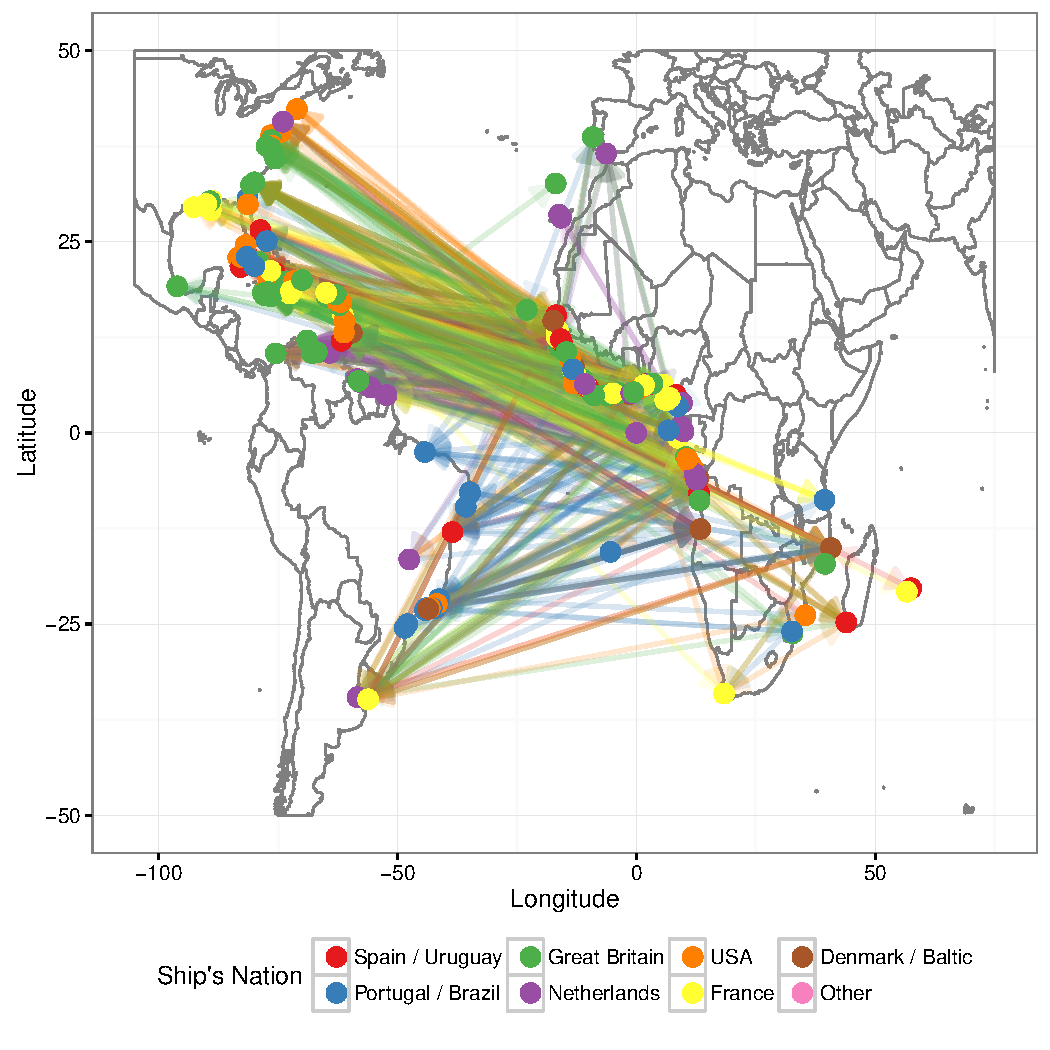
\includegraphics[width=\maxwidth]{figure/whole_dataset_plot-1} \caption[The entire network of completed slave ship trips from Africa to the Americas from 1525 - 1864]{The entire network of completed slave ship trips from Africa to the Americas from 1525 - 1864.}\label{fig:whole_dataset_plot}
\end{figure}


\end{knitrout}


\par The next visualization, in \autoref{fig:biggest_year}, shows the structure of the slave trade network in its busiest year, 1807.  This was the year with the largest number of slaves ships arriving in the Americas.  There were 275 ships that sold slaves in the Americas that year, and 64,109 Africans were sold into slavery that year. And since the database also contains information on how many slaves embarked in Africa, we also know that 73,215 people began those journeys: 9106 Africans died along the way. Interestingly, 1807 was also the year that both Great Britain and the United States made the slave trade illegal.\footnote{See \url{https://en.wikipedia.org/wiki/Abolition_of_slavery_timeline} for more.} We can also see from the plot that the countries' patterns of slave trade are very well-establish 282 years after the first slave ships arrived in the Americas in 1525. British ships travelled primarily to the Caribbean, with some sales in the southern United States, while Portuguese ships only sold slaves in Brazil, and the United States ships sold slaves almost exclusively in Charleston, SC and New Orleans, LA. 

\begin{knitrout}
\definecolor{shadecolor}{rgb}{0.969, 0.969, 0.969}\color{fgcolor}\begin{figure}[h]
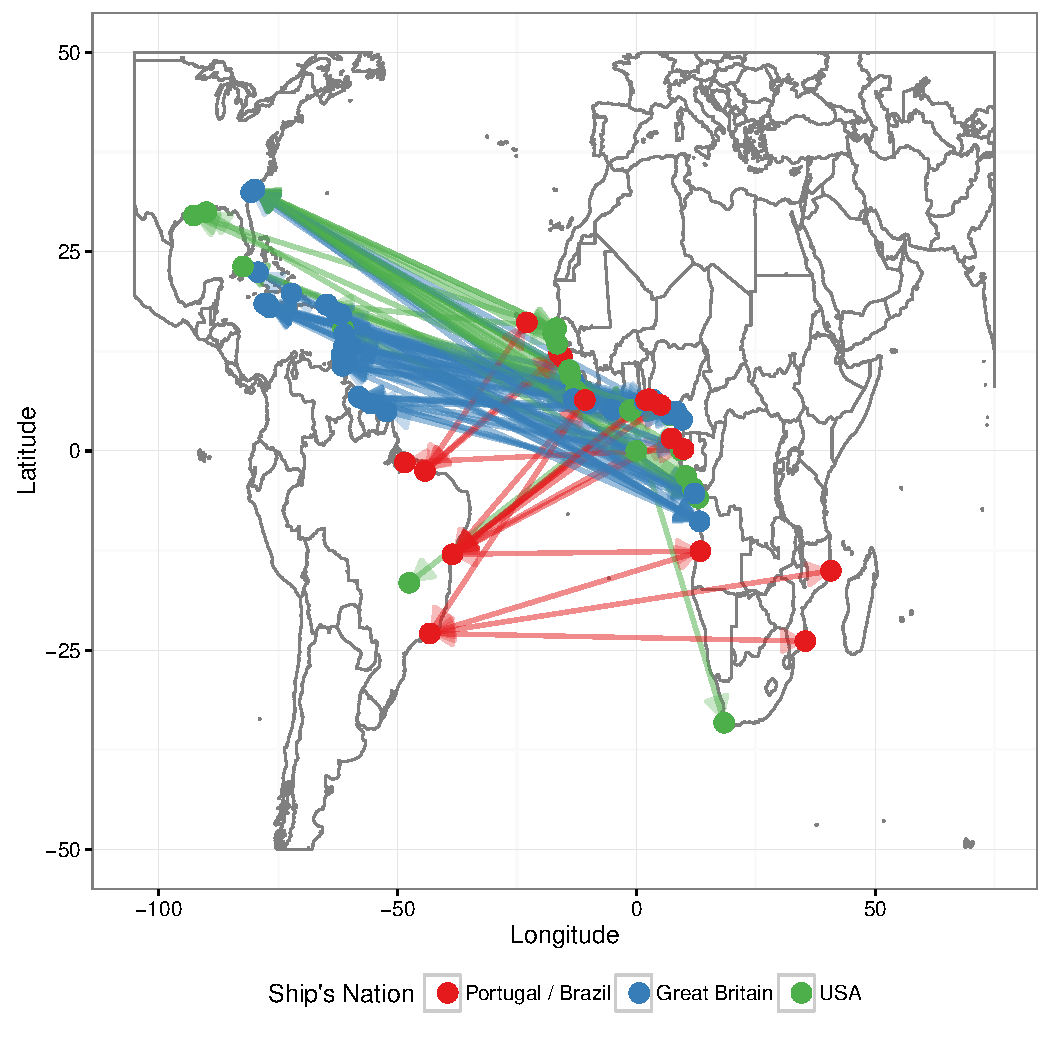
\includegraphics[width=\maxwidth]{figure/biggest_year-1} \caption[Slave trade in 1807, the year with the most slave ships arriving in the Americas]{Slave trade in 1807, the year with the most slave ships arriving in the Americas.}\label{fig:biggest_year}
\end{figure}


\end{knitrout}

\par British ships also made more trips than any other country in the slave trade. From 1562 to 1809 (a period of 247 years), British ships made 7,585 trips carrying over 2.1 \emph{million} Africans, and selling over 1.8 million into slavery, with nearly 300,000 total deaths along the way. On average, a British slave ship carried about 283 Africans, 39 of which died along the way. From the visualization of Great Britain's participation in the slave trade in \autoref{fig:gb}, we see that the vast majority of the British ships made voyages in the $18^{th}$ century. The British empire was extremely influential, and their ships sold Africans into slavery everywhere in the Americas: from New York in the United States, to Montevideo in Uruguay, and almost everywhere with a port in between. The only noticeable gap exists in Brazil, where the Portuguese had a near monopoly on the slave trade.

\begin{knitrout}
\definecolor{shadecolor}{rgb}{0.969, 0.969, 0.969}\color{fgcolor}\begin{figure}[h]
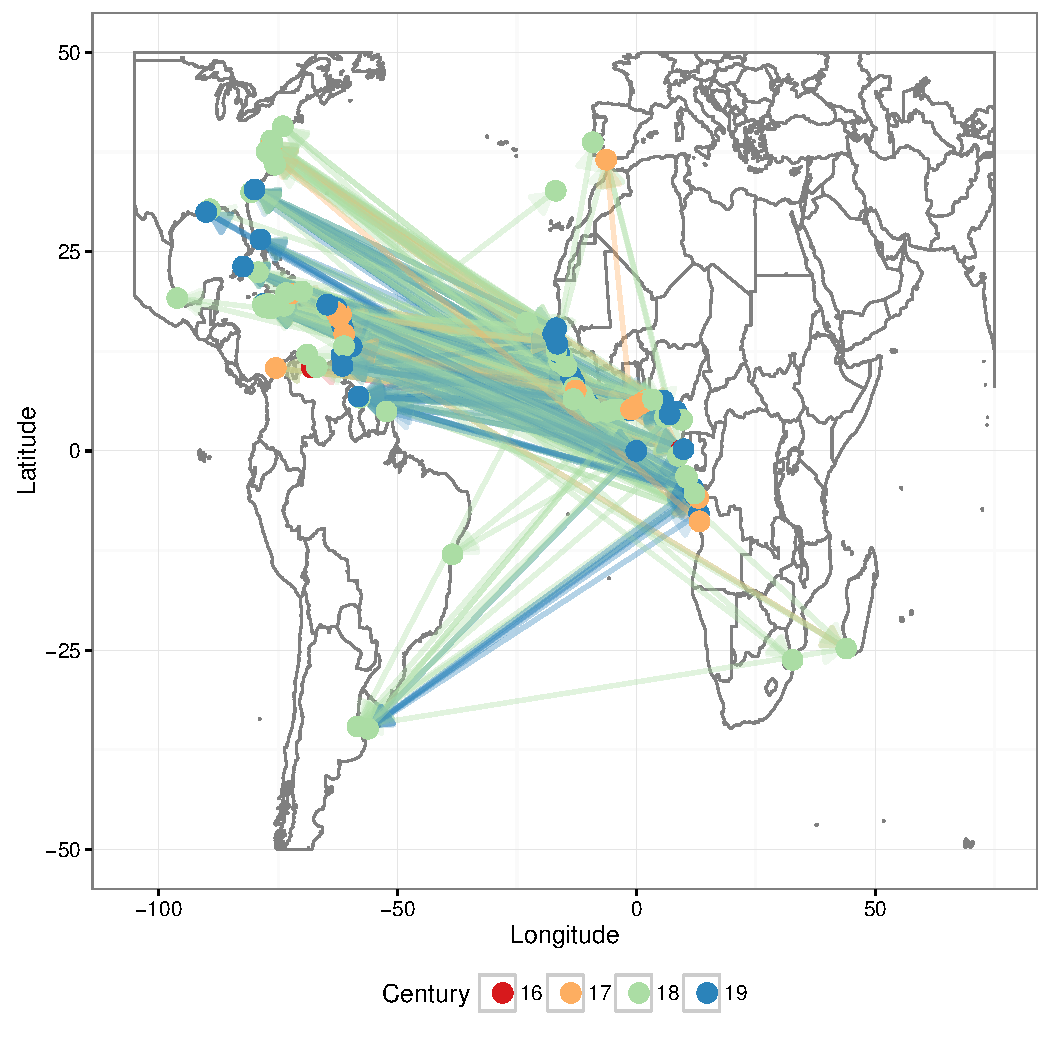
\includegraphics[width=\maxwidth]{figure/gb-1} \caption[All slave trade voyages by British ships, 1562-1809]{All slave trade voyages by British ships, 1562-1809. Color represents the century in which the ship departed Africa with slaves.}\label{fig:gb}
\end{figure}


\end{knitrout}

The second largest participant in the slave trade was the country of Portugal. Portuguese ships began travelling to Africa to buy and sell slaves in 1525 and they did not stop until 1854, a span of 329 years. Portugal forced Africans into slavery for 90 years \emph{longer} than the United States of America has been a country. There have only been 179 years since they outlawed it, and only 161 years since Portugal actually stopped that practice. The impact of this is almost unimaginable. Over 1.9 \emph{million} Africans were taken by the Portuguese, and over 1.7 million were sold into slavery in the Americas, with 200,491 dying during the ocean crossing. The map of the Portuguese slave trade is given in in \autoref{fig:portugal}. The most Portuguese slave voyages occurred in the $19^{th}$ century, with 3,249 slave ship trips across the Alantic in the years 1800-1854. In those 54 years, over 1.3 \emph{million} Africans were forced across the ocean and into slavery, with 124,280 perishing along the way. The Portuguese did over two-thirds of their slave trading in the last 54 of the 329 years they participated. It's easy to imagine that it would have gotten much worse if slave trading had been outlawed later. 
 
\begin{knitrout}
\definecolor{shadecolor}{rgb}{0.969, 0.969, 0.969}\color{fgcolor}\begin{figure}[h]
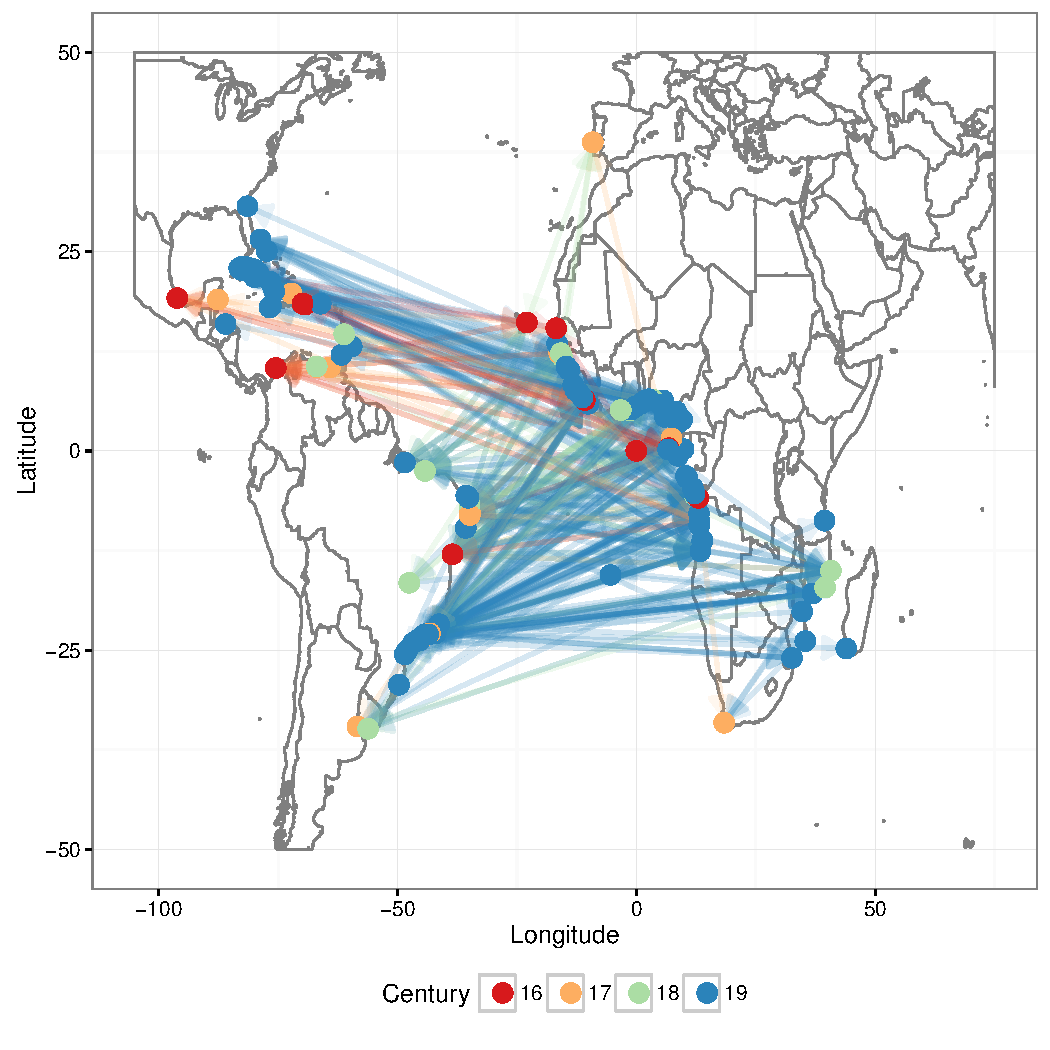
\includegraphics[width=\maxwidth]{figure/portugal-1} \caption[Slave trading voyages by Portuguese ships from 1525-1854]{Slave trading voyages by Portuguese ships from 1525-1854. Color represents the century in which the ship departed Africa with slaves.}\label{fig:portugal}
\end{figure}


\end{knitrout}




\par For British ships overall, about 13.7\% of all Africans died before even reaching the port where they were sold into slavery. This is comparable to ships from Spain, the Netherlands, France, and Denmark, which all had death rates of about 13.6\%, 14.0\%, 13.3\%, and 13.9\%, respectively.  Portuguese ships had the smallest rate of journey deaths, at about 10.1\%, while the American (USA) ships had the highest death rate, at about 16.3\%. In the next visualization, \autoref{fig:slaves_usa}, the points the represent the trading ports are sized by the number of slaves embarked if a departure port or disembarked if a port of slave sale. Most of the points in Africa look bigger than the ports in the Americas, demonstrating the 16.3\% rate of deaths. We also see that the U.S.-owned slave ships did not only sell slaves in the United States. The majority of them, like the British ships, sold slaves in the Caribbean and not in the U.S. All in all, American ships were responsibe for forcing 141,050 Africans overseas and into slavery, with 22,955 dying on the voyage. And, of the 118,095 slaves sold into slavery by American ships, 30,754 of them actually ended up in the United States, while the rest were sold into slavery in the Caribbean and South America.

\begin{knitrout}
\definecolor{shadecolor}{rgb}{0.969, 0.969, 0.969}\color{fgcolor}\begin{figure}[h]
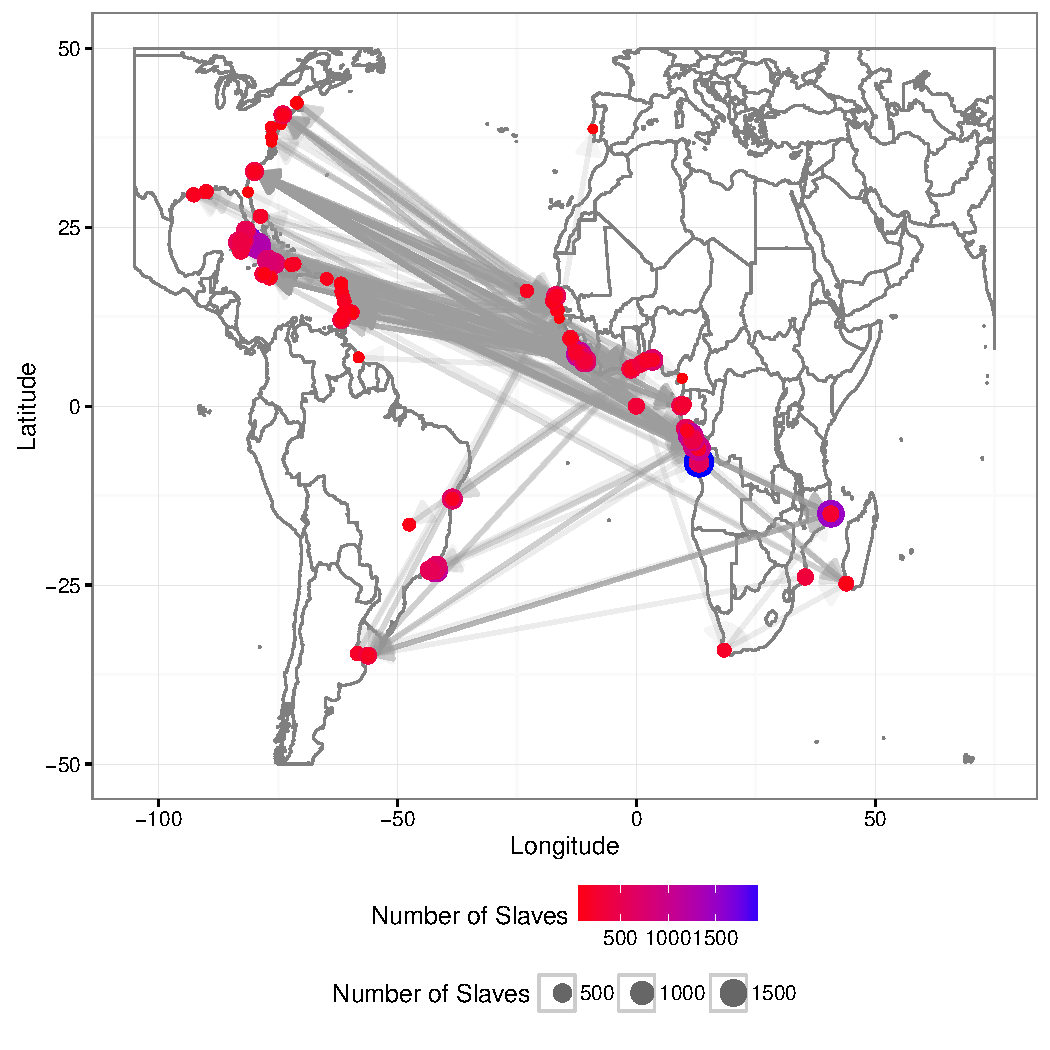
\includegraphics[width=\maxwidth]{figure/slaves_usa-1} \caption[All slave trade ship voyages by U]{All slave trade ship voyages by U.S. ships. Size and color of points represents the number of slaves embarked and disembarked on each voyage.}\label{fig:slaves_usa}
\end{figure}


\end{knitrout}

\par Next I explore the evolution of the slave trade over time. In the first twenty-five years of slaves being sold in the Americas, from 1525-1550, there were only two voyages that arrived. Both were Portuguese ships carrying 300 slaves from S\~{a}o Tom\'{e} in the Gulf of Guinea to the Caribbean. In \autoref{fig:first_years} the first 75 years of voyages, from 1525 to 1600 are shown. There are 98 voyages in these first years, taking 20,951 Africans from their homes and selling 15,322 of them into slavery, with 5,629 dying during the trip across the Atlantic. The only countries participating in in the slave trade in these first years are Spain, Portugal, and Great Britain, and they are only embarking and disembarking at 20 different ports: ten in Africa and ten in the Americas. We can see that Portugal had not yet focused on selling slaves exclusively in Brazil, and the Spanish only sold slaves in modern-day Venezuela. 

\begin{knitrout}
\definecolor{shadecolor}{rgb}{0.969, 0.969, 0.969}\color{fgcolor}\begin{figure}[h]
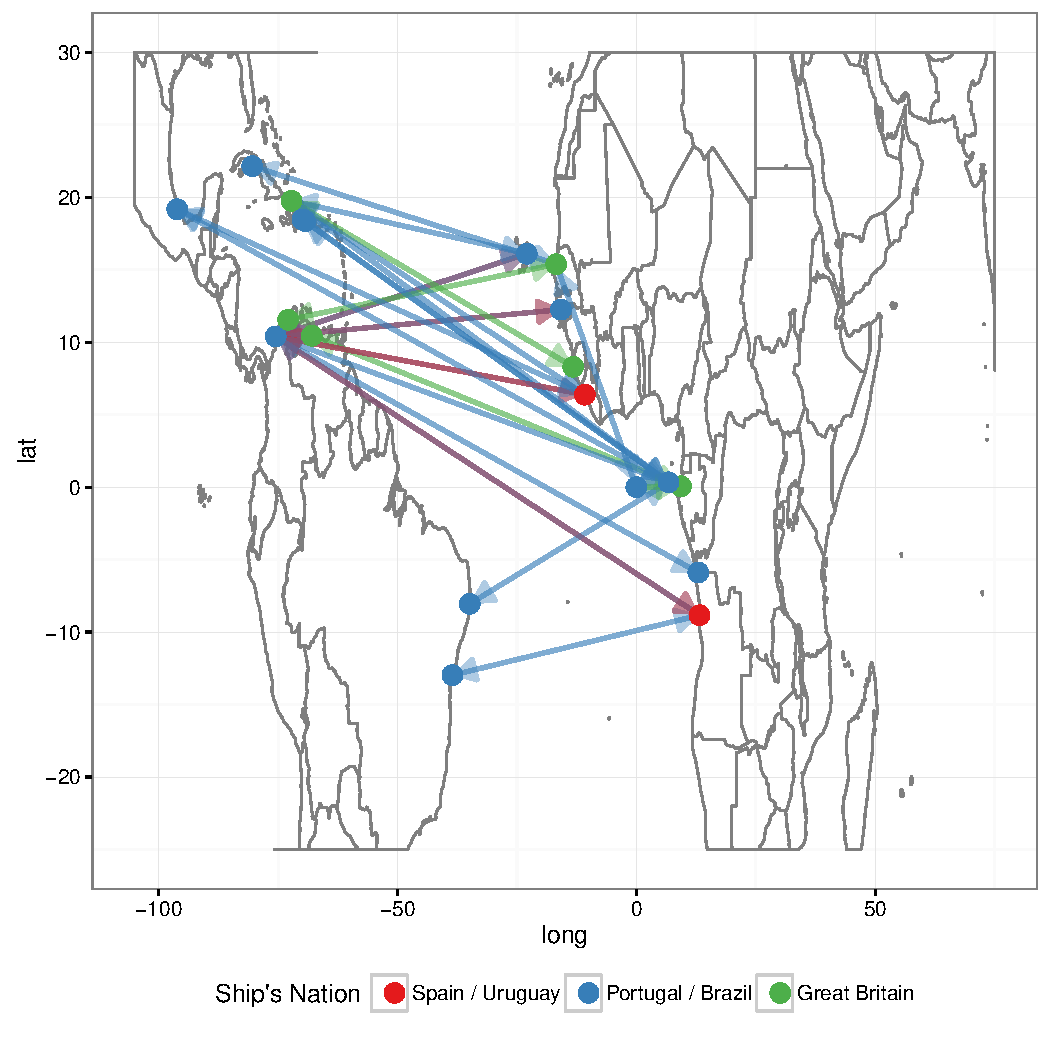
\includegraphics[width=\maxwidth]{figure/first_years-1} \caption[All ships arriving in the Americas in the first 75 years of the slave trade, from 1525-1600]{All ships arriving in the Americas in the first 75 years of the slave trade, from 1525-1600.}\label{fig:first_years}
\end{figure}


\end{knitrout}

\par I also consider the last years of the slave trade. The last year of the slave trade was 1864, and only one ship sold slaves in the Americas that year: a French ship carried 673 Africans from the Congo River area and sold them into slavery in Cuba despite the fact that the slave trade was outlawed in France over 40 years prior in 1818. The last country in the dataset to abolish the slave trade was Portugal, in 1836, yet the slave trade continued for almost two decades more, albeit at a much slower pace. The American ships that were still trading after 1807 were able to do so because the slave trade ban in the U.S. technically only prohibited import of new slaves to the United States. American slave ships still participated in the slave trade by mostly avoiding ports in US territory, selling slaves in the Caribbean and South America instead. This is shown in \autoref{fig:us1808}, with the years of disembarkation and embarkation of slaves printed using the \texttt{label} aesthetic. There is some over-plotting of the labels, but we can see that most of the slave trade routes still being run by US ships after the ban end with slaves being sold in Brazil and in Cuba, where the Portuguese slave traders were ever-present. 

\begin{knitrout}
\definecolor{shadecolor}{rgb}{0.969, 0.969, 0.969}\color{fgcolor}\begin{figure}[h]
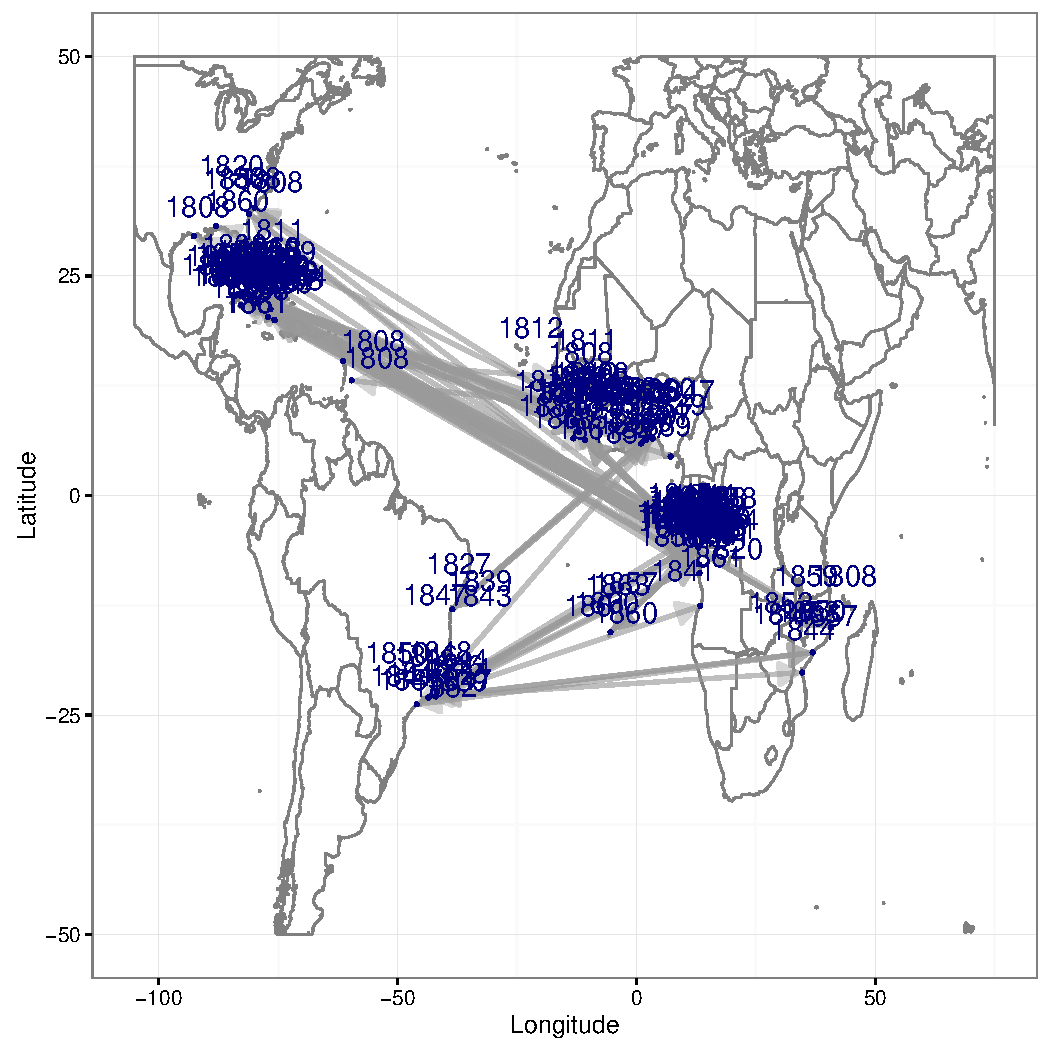
\includegraphics[width=\maxwidth]{figure/us1808-1} \caption[All US ships still participating in the slave trade after its ban in the US in 1807]{All US ships still participating in the slave trade after its ban in the US in 1807.}\label{fig:us1808}
\end{figure}


\end{knitrout}

\par Next, I look at the years after Portugal banned the slave trade, from 1837 to the last year in the data, 1864, for all countries.  There were 778 trans-Atlantic slave trade voyages in that time, and they are shown in \autoref{fig:postban}. Most of these are Portuguese ships, with US and Spanish ships close behind, and nearly all of the trips are to Brazil and the Caribbean.  Interestingly, the most prolific slave trading country, Great Britain, does not appear at all, suggesting that they were most successful in enforcing their bans on slave trade. In fact, the last year that British ships participated in the slave trade was 1810, with only one voyage that year. There were 33 other voyages after the ban, all landing in the Americas in 1808. Given the time it takes to travel across the Atlantic by ship, it is probable that most of those 33 trips began before the slave trade was made illegal. Other countries were nowhere near as good as enforcing their bans on the slave trade. 

\begin{knitrout}
\definecolor{shadecolor}{rgb}{0.969, 0.969, 0.969}\color{fgcolor}\begin{figure}[h]
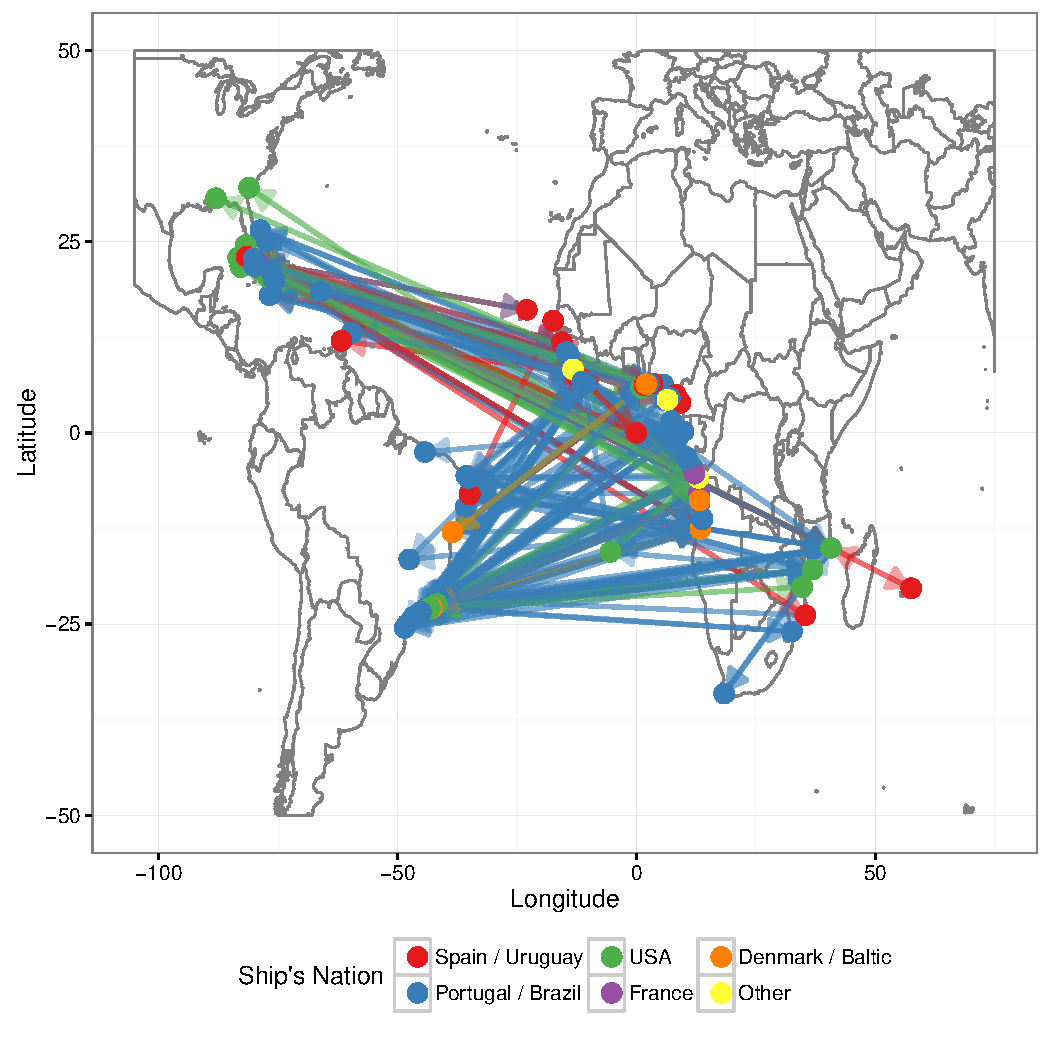
\includegraphics[width=\maxwidth]{figure/postban-1} \caption[All slave trade expeditions that took place after the practice was outlawed in all of the countries that participated]{All slave trade expeditions that took place after the practice was outlawed in all of the countries that participated.}\label{fig:postban}
\end{figure}


\end{knitrout}

\par Finally, I look at the trans-Atlantic slave trade as a traditional network, ignoring the geographical locations of the ports, in order to see which ports played the most central roles in the slave trade. For this visualization I explore a country that we have not yet seen by itself: Spain. Spanish ships made 444 total trips from 1593 to 1859, taking 142,645 people from Africa and selling 123,186 of them into slavery, with 19,459 people dying on the voyages. In \autoref{fig:spain}, I used the Fructerman-Reingold force-directed layout to arrange the nodes and I sized the width of the lines according to the number of slaves on a voyage using the \texttt{linewidth} aesthetic option.% \citep{fruchterman}.
I also labeled a select number of port names in order to see which were most important in the Spanish slave trade network.  The most common points of slave sale are the port of Havana in Cuba, and all other ports in Cuba, as well as the port of Cartagena in Colombia and unspecified ports in Sierra Leone. The frequency of trips \emph{to} Sierra Leone is unusual. As Sierra Leone is a country on the west coast of Africa, I would have expected it to be a port of embarkation instead of a point of disembarkation. The `from' ports of trips taking slaves to Sierra Leone, however, are also in Africa. This suggests that many Spanish slaving ships profited by taking Africans from all over the continent to Sierra Leone to then be sold to another ship's owner and taken across the Atlantic. 

\begin{knitrout}
\definecolor{shadecolor}{rgb}{0.969, 0.969, 0.969}\color{fgcolor}\begin{figure}[h]
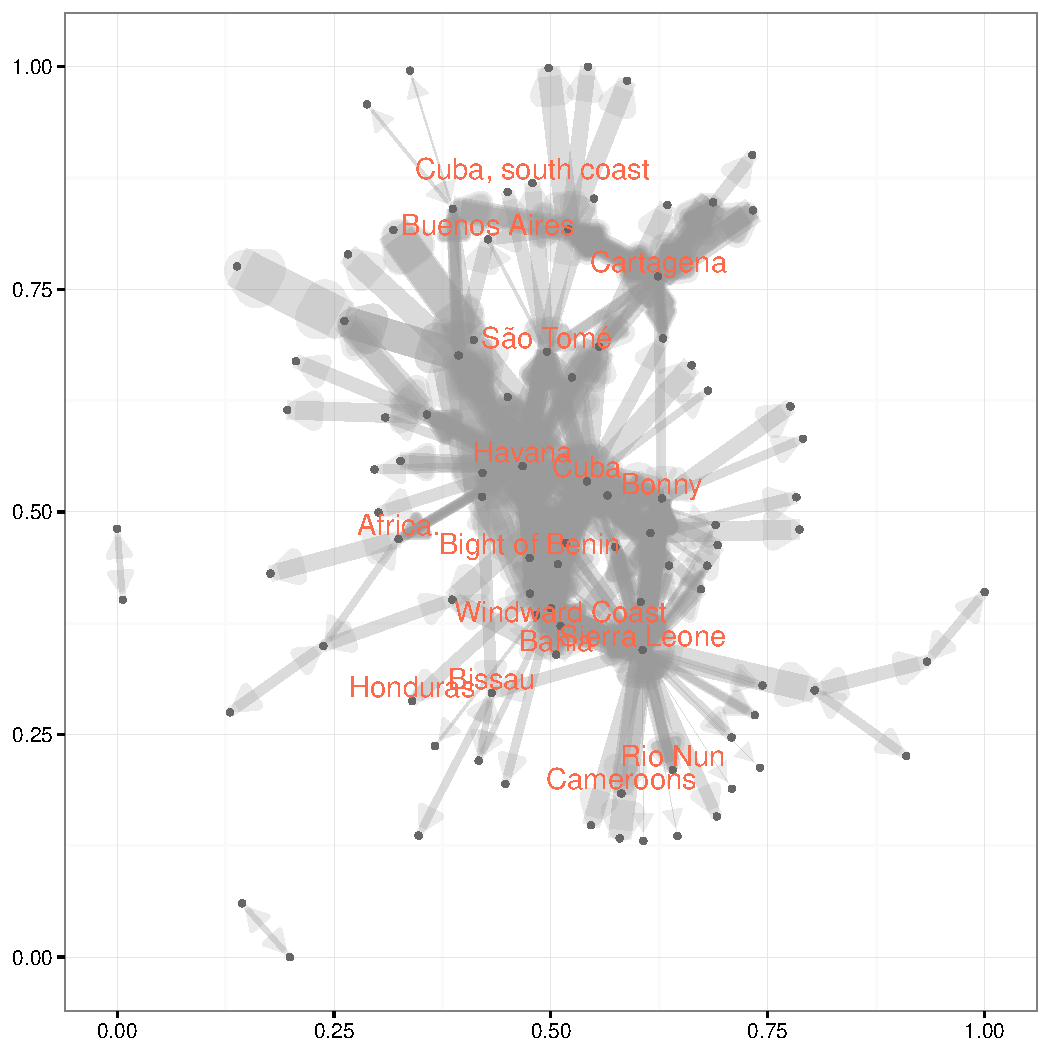
\includegraphics[width=\maxwidth]{figure/spain-1} \caption[The network of slave trade by Spanish ships from 1593 to 1859]{The network of slave trade by Spanish ships from 1593 to 1859.}\label{fig:spain}
\end{figure}


\end{knitrout}

\section*{Conclusion}

After exploring the Trans-Atlantic Slave Trade Database, I have a much deeper understanding of the slave trade than any history class has ever given me. Being able to see the voyages on the map and being able to look at individual voyages in the data helped to comprehend just how massive the slave trade was. Seeing the size of the points on the map shrink after crossing the ocean and seeing the huge numbers of trips made to the Caribbean really brought the horror of the slave trade to the forefront of my mind. Viewing the slaving voyages as a network was an incredibly effective way to visualize the slave trade data. 

\par The last slaving ship disembarked in Cuba 151 years ago, which sounds like a very long time ago, until you realize that the trans-Atlantic slave trade persisted for more than twice that amount of time.  Because of this, the slave trade has left a lasting impact on the Americas. For instance, in the United States of America, December 6, 2015, marked the $150^{th}$ anniversary of the abolition of slavery becoming law, yet there are still inequities in the way African-Americans are treated every day in in the U.S. Thus, the impact of the trans-Atlantic slave trade cannot be ignored, especially in light of this important anniversary. These visualizations are sure to bring that impact to the forefront of the viewer's mind. 
%----------------------------------------------------------------------------------------
%	REFERENCE LIST
%----------------------------------------------------------------------------------------
%\bibliographystyle{abbrv}
%\bibliography{ASA_SCSG_Paper}
\section*{Further Reading}
To view more visualizations of the slave voyages data, go to \url{www.slavevoyages.org/voyage/search} and explore the Custom Graphs and Animation tabs. The animations by Slate magazine and Georgetown University can be found at \url{www.slate.com/articles/life/the_history_of_american_slavery/2015/06/animated_interactive_of_the_history_of_the_atlantic_slave_trade.html} and \url{http://mcb226.github.io/SlaveTrade/}, respectively. Finally, Hadley Wickham’s book \emph{ggplot2: Elegant Graphics for Data Analysis} contains much more information on the \texttt{ggplot2} package and how it works, and the documentation of \texttt{geomnet} contains more examples and details.

%----------------------------------------------------------------------------------------

\end{document}
